\documentclass[
	12pt,
	a4paper,
	oneside,
	pagesize=auto,	
  version=last, % Koma Script version
	toc=listof, % add tables and figures to toc
  bibliography=totoc % add bibliography to toc
	]{scrartcl}

% language
\usepackage[utf8]{inputenc}
\usepackage[T1]{fontenc}
\usepackage{csquotes}
\usepackage[ngerman]{babel}

\input{preamble/styles.tex}
% linked toc
\usepackage{hyperref}
\hypersetup{
  colorlinks,
  citecolor=black,
  filecolor=black,
  linkcolor=black,
  urlcolor=black
}

% biblatex
\usepackage[
  backend=biber,
  style=authoryear,
  %autocite=footnote,
  %maxnames=4,
  %ibidpage=true,
]{biblatex}
\addbibresource{literature.bib}

% configure colors
\usepackage{xcolor}

\usepackage{xpatch}
\xpatchbibdriver{online}
{\printtext[parens]{\usebibmacro{data}}}
{\iffieldundef{year}{}{\printtext[parens]{\usebibmacro{data}}}}{}{}

\usepackage{xcolor}

% listings package with language configs
\usepackage{listings}
\usepackage[dvipsnames]{xcolor}


% Default style for all listings. Among other things, fixes 
\lstset{
	% --- Linenos ---
	numbersep=3pt,                  % how far the line-numbers are from the code
	numberstyle=\tiny\color{gray},
	numbers=left,                   % where to put the line-numbers
	stepnumber=1,                   % the step between two line-numbers. If it is 1 each line will be numbered
	% -- Basics --
	basicstyle=\ttfamily,
	sensitive=true,  % Case-sensitive keywords
	tabsize=4,
	breaklines=true,  % Break lines if too long
	%escapechar=`,
	%escapeinside={<@}{@>},
	% I don't know what keepspaces and columns do, but together, they fix the ugly default listings style.
	columns=fullflexible,
	keepspaces,
	showstringspaces=false,  % Spaces not shown as _
	basicstyle=\ttfamily\footnotesize,
}

% Usage: \begin{lstlisting}[language=notepadpp-xml] ...
\lstdefinelanguage{XML}{
	morestring=[b]",                       % "attribute strings"
	morecomment=[s]{!--}{--},            % <!-- comments -->
	morecomment=[s]{?}{?},               % <? xml instructions ?>
	morekeywords={id}, % tag names (customize)
	keywordstyle=\color{YellowGreen},      % element/tag names
	identifierstyle=\color{NavyBlue},  % attribute names
	stringstyle=\color{Fuchsia},    % attribute values
	commentstyle=\color{ForestGreen},  % XML comments
	moredelim=[s][\color{black}]{>}{<},
	showstringspaces=false,
	breaklines=true
}

% Usage: \begin{lstlisting}[language=notepadpp-xml] ...
\lstdefinelanguage{racketSQL}{
%	language=SQL,
%	morestring=[b]",                   % "attribute strings"
	morecomment=[s]{;;}{;;},           % <;; comments ;;>
	morekeywords={ABSOLUTE,ACTION,ADD,ALLOCATE,ALTER,ARE,AS,ASSERTION,%
		AT,BEGIN,BETWEEN,BIT_LENGTH,BOTH,BY,CASCADE,CASCADED,CASE,CAST,%
		CATALOG,CHAR_LENGTH,CHARACTER_LENGTH,CLUSTER,COALESCE,%
		COLLATE,COLLATION,COLUMN,CONNECT,CONNECTION,CONSTRAINT,%
		CONSTRAINTS,CONVERT,CORRESPONDING,CREATE,CROSS,CURRENT_DATE,%
		CURRENT_TIME,CURRENT_TIMESTAMP,CURRENT_USER,DAY,DEALLOCATE,%
		DEC,DEFERRABLE,DEFERED,DESCRIBE,DESCRIPTOR,DIAGNOSTICS,%
		DISCONNECT,DOMAIN,DROP,ELSE,END,EXEC,EXCEPT,EXCEPTION,EXECUTE,%
		EXTERNAL,EXTRACT,FALSE,FIRST,FOREIGN,FROM,FULL,GET,GLOBAL,%
		GRAPHIC,HAVING,HOUR,IDENTITY,IMMEDIATE,INDEX,INITIALLY,INNER,%
		INPUT,INSENSITIVE,INSERT,INTO,INTERSECT,INTERVAL,%
		ISOLATION,JOIN,KEY,LAST,LEADING,LEFT,LEVEL,LIMIT,LOCAL,LOWER,%
		MATCH,MINUTE,MONTH,NAMES,NATIONAL,NATURAL,NCHAR,NEXT,NO,NOT,NULL,%
		NULLIF,OCTET_LENGTH,ON,ONLY,ORDER,ORDERED,OUTER,OUTPUT,OVERLAPS,%
		PAD,PARTIAL,POSITION,PREPARE,PRESERVE,PRIMARY,PRIOR,READ,%
		RELATIVE,RESTRICT,REVOKE,RIGHT,ROWS,SCROLL,SECOND,SELECT,SESSION,%
		SESSION_USER,SIZE,SPACE,SQLSTATE,SUBSTRING,SYSTEM_USER,%
		TABLE,TEMPORARY,THEN,TIMEZONE_HOUR,%
		TIMEZONE_MINUTE,TRAILING,TRANSACTION,TRANSLATE,TRANSLATION,TRIM,%
		TRUE,UNIQUE,UNKNOWN,UPPER,USAGE,USING,VALUE,VALUES,%
		VARGRAPHIC,VARYING,WHEN,WHERE,WRITE,YEAR,ZONE,%
		AND,ASC,avg,CHECK,COMMIT,count,DECODE,DESC,DISTINCT,GROUP,IN,% FF
		LIKE,NUMBER,ROLLBACK,SUBSTR,sum,VARCHAR2,% FF
		MIN,MAX,UNION,UPDATE,% RF
		ALL,ANY,CUBE,CUBE,DEFAULT,DELETE,EXISTS,GRANT,OR,RECURSIVE,% DJ
		ROLE,ROLLUP,SET,SOME,TRIGGER,VIEW},% DJ,
	keywordstyle=\bfseries,      % element/tag names
%	identifierstyle=\color{NavyBlue},  % attribute names
	stringstyle=\color{Fuchsia},    % attribute values
	commentstyle=\color{ForestGreen},  % XML comments
%	moredelim=[s][\color{black}]{>}{<},
%	showstringspaces=false,
	breaklines=true
	}

% Usage: \begin{lstlisting}[language=racket] ...
\lstdefinelanguage{racket} {
	% -- Comments --
	%morecomment=[l]{//},
	%morecomment=[s]{/*}{*/},
	morecomment=[l]{;},         % Inline comments start with ;
	morecomment=[s]{\#|}{|\#},  % Block comments are done with #|  |#
	commentstyle={\color{ForestGreen}\slshape\sffamily},
	% -- Strings --
	morestring=[b]",
	stringstyle=\color{red},
	% --- Literal replacements ---
	literate=%
	%	{lambda}{{$\lambda$}}1
		{->}{{$\rightarrow$}}1
		{*}{{$\times$}}1,
	% -- Keywords (I got these from a vague French website; Racket seems to have no lstlisting style defined anywhere) --
	classoffset=1,
		morekeywords={
			define, define-syntax, define-macro, define-datatype, lambda, define-stream, stream-lambda
		},
		keywordstyle=\color{purple},
	classoffset=2,
		morekeywords={
			begin, call-with-current-continuation, call/cc, call-with-input-file, call-with-output-file, 
			cases, cond, do, else, for-each, if,
			let*, let, let-syntax, letrec, letrec-syntax,
			define-context, define-controller, Integer, Boolean, get, when-required, when-provided,
			maybe_publish, require, submod, or/c, ->, \#\%module-begin, always_publish, with-syntax, define-struct/contract, syntax-case, define/contract,
			let-values, let*-values,
			module, provide,
			and, or, not, 
			delay, force,
			\#`, \#',
			null, cons, car, cdr, cadr, caddr,
			\#lang, implement, begin-for-syntax, rename-out,
			quasiquote, quote, unquote, unquote-splicing,
			map, filter, foldl, syntax, syntax-rules, eval, environment, query 
		},
		keywordstyle=\color{blue},
	classoffset=3,
		morekeywords={import, export},
		keywordstyle=\color{green},
	classoffset=0,
	alsoletter={',`,-,/,>,<,\#,\%},
	moredelim=**[is][\color{lightgray}]{<<@<<}{>>@>>},
	moredelim=**[is][\itshape\color{OliveGreen}]{<<;<<}{>>;>>},
}

% Inline racket
\newcommand{\ir}[1]{\lstinline[basicstyle=\ttfamily\small,language=racket]{#1}}


% acronym
\usepackage[printonlyused]{acronym}

% saves current page roman/arabic number
\usepackage{etoolbox}
\newcounter{savedpage}

\usepackage{enumitem}
\usepackage{amsmath}

%Tabellen
\usepackage{booktabs}
%Tabelle
\usepackage{multirow,makecell}
\usepackage{ltablex}
\usepackage{booktabs}
\newcolumntype{L}[1]{>{\RaggedRight}p{#1}} 
\newcolumntype{C}[1]{>{\centering\arraybackslash}p{#1}} 

\usepackage{array}

% configure graphicx
\usepackage{graphicx}
\graphicspath{{./assets/images}}

% Configure Tables
\usepackage[normalem]{ulem}
\useunder{\uline}{\ul}{}
\usepackage{lscape}


% configure captions
%\usepackage{caption}
%\captionsetup{width=0.8\textwidth}

% configure dates
\usepackage[useregional=numeric]{datetime2}

% configuration

% paper details
%-----------------------------------------------------------------------------------
\newcommand*{\paperType}{Assignment}
% title
\newcommand*{\paperTitle}{Datenbank-Programmierung}
% subject
\newcommand*{\paperSubject}{PRG24-LB-06}
% module
\newcommand*{\paperModuleShort}{PRG24}
\newcommand*{\paperModule}{\paperModuleShort - Programmierparadigmen}
% lecturer
\newcommand*{\paperLecturerLabel}{Betreuerin}
\newcommand*{\paperLecturer}{Prof. Dr. Andrea Herrmann}
% submission date
\newcommand*{\registrationDate}{08.05.2026}
% name
\newcommand*{\authorName}{Namen der Autoren}
% address
\newcommand*{\authorStreet}{Straßenname Hausnummer}
\newcommand*{\authorCity}{PLZ Ort}
% student number
\newcommand*{\studentNo}{Matrikelnumemr}
% course of studies
\newcommand{\courseOfStudies}{Software Engineering - Bachelor of Engineering (B. Eng.)}
% email 
\newcommand*{\authorEmail}{\href{mailto:Emailadresse}{Emailadresse}}
% headnote
\newcommand*{\paperHeadnote}{\paperType\space\paperModuleShort\space\textemdash\space\paperTitle}

%-----------------------------------------------------------------------------------


% glossary
%\usepackage[
%nonumberlist,
%toc
%]{glossaries}
%\usepackage[acronym,symbols]{glossaries}
%\usepackage{glossaries}
%\makenoidxglossaries
%% Glossar
\newglossaryentry{Entitaet}
	{name=Entität,
		description={Eine Entität, "ist ein Element der Datenwelt, welches ein reales oder gedankliches Einzelphänomen in einem betrachteten Realitätsausschnitt repräsentiert." (\cite{gehringWirtschaftsinformatik2022}: 787)},
	}

\newglossaryentry{Entitaets-Beziehung}
 	{name=Entitäts-Beziehung,
 		description={"Eine [Entitäts-]Beziehung (engl. relationship) ist eine logische Verknüpfung zwischen zwei oder mehreren Entitäten bzw. Entitätstypen." (\cite{gehringWirtschaftsinformatik2022}: 788)}
	}
	
\newglossaryentry{Entitaets-Typ}
	{name=Entitäts-Typ,
		description={"Ein Entitätstyp (oder Entitätsmenge, engl. entity set) fasst alle Entitäten zusammen, die durch gleiche Merkmale, nicht notwendigerweise aber durch gleiche Merkmalsausprägungen, charakterisiert werden." (\cite{gehringWirtschaftsinformatik2022}: 788)}
	}
	
\newglossaryentry{Assoziation}
{name=Assoziation,
	description={Im ERM Modell gibt eine "Assoziation [...] an, wie viele Entitäten eines Entitätstyps [A] einer beliebigen Entität des Entitätstyps [B] zugeordnet sein können." (\cite{gehringWirtschaftsinformatik2022}: 788)}
}

\newglossaryentry{Normalisierung}
{name=Normalisierung,
	description={}
} did not use glossary in this work

\begin{document}

% title page
\thispagestyle{empty}

\begin{center}
  \LARGE{AKAD Bildungsgesellschaft mbH}\\
  \large{\courseOfStudies}\\[3em]
  
\includegraphics[width=0.4\textwidth]{assets/Akad_University_Logo.png}\\[5em]
  \textbf{\large{\paperType}}\\
  \large{\paperModule}\\[2em]
  \Large{\textbf{\paperTitle}}\\
  \large{\paperSubject}
\end{center}
\vfill
\begin{small}
  \begin{tabular}{ll}
    Vorgelegt von:       &                            \\
    Name:                & \authorName              \\[-1ex]
    Adresse:             & \authorStreet, \authorCity \\
    Imma. Nr.:           & \studentNo                 \\[-1ex]
    Email:               & \authorEmail \\
    Anmeldedatum:        & \registrationDate          \\[-1ex]
    Abgabedatum:         & \today                     \\[-1ex]
    \paperLecturerLabel: 		 & \paperLecturer
  \end{tabular}
\end{small}
\clearpage

\pagenumbering{Roman}

% ToC etc.
\tableofcontents
\clearpage
\listoffigures
\clearpage
\listoftables
\clearpage
%\input{content/acronyms}
%\clearpage

\setcounter{savedpage}{\value{page}}

\pagenumbering{arabic}


% --- LOAD SECTIONS ---
%\section{Modellierung eines Datenmodells für Datenbanksysteme}

\subsection*{Ziel}
Ein \textbf{Datenmodell} beschreibt die Struktur, Beziehungen und Regeln der Daten, 
die in einem IT-System gespeichert und verarbeitet werden. 
Das Ziel besteht darin, eine \textbf{konsistente, redundanzfreie und performante Abbildung der Realwelt} in Datenbankform zu schaffen.

\subsection*{1. Phasen der Datenmodellierung}

\subsubsection*{1.1 Konzeptionelles Datenmodell (Fachliches Modell)}
\begin{itemize}
	\item \textbf{Ziel:} Abbilden der realen Welt aus Sicht des Fachbereichs.
	\item \textbf{Werkzeug:} Entity-Relationship-Diagramm (ERD) oder UML-Klassendiagramm.
	\item \textbf{Elemente:}
	\begin{itemize}
		\item \textbf{Entitäten} (z.\,B. \textit{Kunde}, \textit{Produkt}, \textit{Bestellung})
		\item \textbf{Attribute} (z.\,B. \textit{Kundenname}, \textit{Preis})
		\item \textbf{Beziehungen} (z.\,B. \textit{Kunde gibt Bestellung auf})
	\end{itemize}
\end{itemize}
\textbf{Ergebnis:} Ein fachliches, technologieunabhängiges ER-Diagramm.

\subsubsection*{1.2 Logisches Datenmodell}
\begin{itemize}
	\item \textbf{Ziel:} Präzisierung des konzeptionellen Modells auf Datenbankebene.
	\item \textbf{Werkzeug:} Logisches ER-Diagramm (z.\,B. Chen- oder Crow’s-Foot-Notation).
	\item \textbf{Schritte:}
	\begin{itemize}
		\item Definition von Primär- und Fremdschlüsseln.
		\item Festlegung der Beziehungstypen (1:1, 1:n, m:n).
		\item Normalisierung (mindestens bis zur 3. Normalform, oft 3NF oder BCNF).
	\end{itemize}
\end{itemize}
\textbf{Ergebnis:} Ein strukturierter, logischer Entwurf, der sich direkt in Tabellen übersetzen lässt.

\subsubsection*{1.3 Physisches Datenmodell}
\begin{itemize}
	\item \textbf{Ziel:} Umsetzung in einem konkreten Datenbanksystem.
	\item \textbf{Werkzeug:} SQL-DDL-Skripte (\texttt{CREATE TABLE ...}), Datenbank-Design-Tools.
	\item \textbf{Schritte:}
	\begin{itemize}
		\item Definition von Datentypen (z.\,B. \texttt{VARCHAR(255)}, \texttt{INT}, \texttt{DATE})
		\item Indizes, Constraints, Trigger
		\item Performance-Überlegungen (Partitionierung, Denormalisierung, Materialized Views)
		\item Physische Speicheroptionen (z.\,B. Tablespaces, Sharding)
	\end{itemize}
\end{itemize}
\textbf{Ergebnis:} Ein lauffähiges Datenbankschema, bereit zur Implementierung.

\subsection*{2. Vorgehensweise in der Praxis}
\begin{enumerate}[label=\arabic*.]
	\item \textbf{Anforderungsanalyse:} Erheben, welche Informationen das System speichern und verarbeiten muss.
	\item \textbf{Erstellen des konzeptionellen Modells:} Entitäten, Attribute und Beziehungen skizzieren.
	\item \textbf{Validierung mit Fachanwendern:} Prüfen, ob das Modell die Realität korrekt abbildet.
	\item \textbf{Überführung ins logische Modell:} Schlüsselfelder, Kardinalitäten und Normalisierung definieren.
	\item \textbf{Erstellung des physischen Modells:} Umsetzung für ein konkretes DBMS (z.\,B. PostgreSQL).
	\item \textbf{Optimierung und Pflege:} Performance-Tuning, Versionierung, Änderungsmanagement.
\end{enumerate}

\subsection*{3. Tools zur Datenmodellierung}
\begin{tabular}{@{}p{4cm}p{10cm}@{}}
	\toprule
	\textbf{Typ} & \textbf{Beispiele} \\ \midrule
	Professionelle Werkzeuge & ER/Studio, SAP PowerDesigner, Oracle SQL Developer Data Modeler \\
	Open Source / Kostenlos & dbdiagram.io, draw.io, Lucidchart, DBeaver, pgModeler \\
	Codebasiert & Prisma (Node.js), SQLAlchemy (Python), Hibernate (Java ORM) \\
	\bottomrule
\end{tabular}

\subsection*{4. Beispiel eines logischen Modells}
Ein einfaches logisches Modell für einen Online-Shop:
\begin{verbatim}
	Kunde (KundenID PK, Name, E-Mail)
	Bestellung (BestellID PK, Datum, KundenID FK)
	Produkt (ProduktID PK, Bezeichnung, Preis)
	Bestellposition (BestellID FK, ProduktID FK, Menge)
\end{verbatim}

\noindent Beziehungen:
\begin{itemize}
	\item Kunde — Bestellung: 1:n
	\item Bestellung — Bestellposition: 1:n
	\item Produkt — Bestellposition: 1:n
\end{itemize}
\section{Einleitung}
\label{sec:Einleitung}
Laut Definition ist \glqq Eine Datenbank ist eine Sammlung von Daten, die untereinander in einer logischen Beziehung stehen und von einem eigenen Datenbankmanagementsystem (Database Management System, DBMS) verwaltet werden\grqq (\cite{kaufmannSQLNoSQLDatenbanken92023}, S.3). Das DBMS ermöglicht idealerweise einen Zugriff durch mehrere Anwendungen oder Endnutzer, welche gleichzeitig, fehlerfrei, schnell und sicher die Informationen aus den Daten abfragen und konfliktfrei verändern können, und das bei minimalem Bedarf an Systemressourcen.

Diese Vorteile einer zentralen Datenverwaltung für mehrere Klienten werden insbesondere deutlich, wenn man das Datenbanksystem mit einer einfachen Dateiverwaltung vergleicht. Hier verwendet jede Anwendung und Endnutzer ein eigenes Dateisystem und physische Ablage auf einem Speichersystem. Redundanzen und Inkonsistenzen entstehen schnell, wenn die gleichen Daten durch Kopieren an einen anderen Speicherplatz übertragen oder redundante Daten nur an einer Stelle verändert werden. Auch ist die logische Struktur der Dateiablage und Codierungen (Dateiformate) individuell auf die Anwendungen abgestimmt, was die Flexibilität bei einer erforderlichen gemeinsamen Datenverarbeitung beeinträchtigt.

Je nach Anwendung werden unterschiedliche Datenbanksysteme eingesetzt, die sich deutlich in der Datenstruktur unterscheiden. In der heutigen Zeit haben sich insbesondere das relationale Modell und No-SQL-Datenbanken (im Bereich von Big-Data) durchgesetzt, während hierarchische Modelle und objektorientierte Modelle (oder Mischformen wie objektrelationale Modelle) weitestgehend verdrängt wurden (\cite{kaufmannSQLNoSQLDatenbanken92023}: 12ff; \cite{gehringWirtschaftsinformatik2022}: 781). Das relationale Modell bietet im Vergleich zu den anderen Modellen insbesondere den Vorteil, dass die Datenkonsistenz sehr gut eingehalten werden kann, da die Datentypen streng einheitlich definiert werden.

Das Vorgehen bei der Erstellung einer Datenbank ist die \textit{Datenbankmodellierung} und verfolgt die Ziele (\cite{schickerDatenbankenUndSQL2025}, S.23) einer
\begin{itemize}[itemsep=3pt]
	%https://www.overleaf.com/learn/latex/Lists#The_itemize_environment_for_bulleted_(unordered)_lists
	\item{geringen Redundanz,} 
	\item{guten Bedienbarkeit und einfachen Erweiterbarkeit,} 
	\item{schnellen Zugriffszeiten,} 
	\item{Konsistenz,}
	\item{und Integrität.}
\end{itemize}

Die Ziele können teils miteinander konkurrieren, sodass es oft nicht möglich ist, alle Ziele gleichsam zu optimieren. Beispielsweise ist vorstellbar, dass aus dem Datenbestand abgeleitete oder berechnete Daten für eine bessere Performance in verarbeiteten Datentypen zusätzlich gespeichert werden. Die eindeutige funktionale Beziehung zu den Rohdaten erzeugt somit eine Redundanz, welche außerdem die Datenkonsistenz im Fehlerfall beeinträchtigen kann. Weiterhin ist es möglich, dass im Sinne einer Redundanz-Optimierung gewisse Attribute, welche in verschiedenen Objekten der Datenbank in identischer Form vorkommen, separat gespeichert werden. Werden nun die Objekte gelöscht, bleiben diese separat gespeicherten Attribute womöglich bestehen, wodurch die referentielle Integrität beeinträchtigt wird, da Datenbestände entstehen, die keinen sinnvollen Bezug mehr zu den eigentlich für die Datenbank wichtigen Datenbeständen haben. Diese Konflikte zeigen die Schwierigkeit bei den Zielstellungen einer Datenbankmodellierung. Es ist daher wichtig, dass die Datenbankmodellierung nicht nur an den bestehenden Bestand von Datensätzen angepasst ist, sondern auch wachsende Anforderungen an die Anzahl der Datensätze sowie zusätzliche Funktionen von Anfang an mitgedacht werden. Die flexible Erweiterbarkeit sollte daher bei potenziell wachsenden Datenbanken stets mitgedacht werden.

\subsection{Problemstellung}
\label{subsection:Problemstellung}
In dieser Arbeit wird die Datenbankmodellierung an einem selbstgewählten Anwendungsfall schrittweise durchgeführt. Beispielhaft wird die Umsetzung eines Datenbankmodells anhand der Carsharing App \glqq TeilAuto Neckaralb\grqq demonstriert, die vom Autor dieser Arbeit regelmä{\ss}ig verwendet wird. Ähnlich anderen Carsharing-Anbietern ermöglicht diese App die zeitlich und örtlich flexible Miete diverser Fahrzeuge und Fahrzeugklassen vom Lastenrad, über das Familienauto bis hin zum Umzugstransporter. Monatlich wird für jede/n Kund:in eine Rechnung erstellt, die die persönlichen Buchungen zusammen mit dem im Vertrag festgelegten Tarif verrechnet. Hierbei können mehrere Kund:innen den gleichen Vertrag besitzen wenn sie diesem als Gruppe (Haushalt, Familie) zugeteilt sind und so einen vergünstigten Gruppen-Tarif erhalten, wobei die Rechnungen weiterhin kund:innenspezifisch erstellt werden. Das Datenmodell soll sowohl die Sichtweise von Kund:innen, als auch dem Carsharing-Anbieter widerspiegeln und es ermöglichen, dass Kund:innen bei Buchungen auf die für sie relevanten Informationen zugreifen können, als auch die Mitarbeitenden des Unternehmens die Informationen erhalten um Kund:innen, Verträge, Abrechnungen und Fahrzeuge zu managen.

\subsection{Ziel und Aufbau der Arbeit}
Das Hauptziel dieser Arbeit ist es, den vollständigen Entwurfsprozess einer Datenbank anhand des Beispiels der Carsharing-Applikation zu erklären und praktisch zu erarbeiten. Zuerst werden in \autoref{section:basics} die theoretischen Grundlagen zur Modellierung relationaler Datenbanken erläutert. Als grundlegende Schritte finden sich hier die Anforderungsanalyse, aus der ein Entity-Relationship-Modell (ERM) konzipiert wird, das die grundlegenden Entitäten, Attribute und Beziehungen grafisch darstellt und die Überführung des ERM in ein in dieser Arbeit gewähltes Relationenmodell, das die Entitätstypen und Beziehungstypen in Tabellen überführt. Es wird gezeigt, durch welche Normalisierungs-Regeln diese Tabellen bezüglich der Ziele einer Datenbankmodellierung optimiert werden können. Anschließend wird im praktischen Teil in \autoref{section:main} das Beispiel der Carsharing-Applikation auf Basis der vorgestellten Modellierungsschritte vollständig entworfen und in der Programmiersprache Racket und dem DBMS SQLite praktisch umgesetzt. Abschließend wird in \autoref{section:summary} die Arbeit zusammengefasst und die Umsetzung kritisch beleuchtet.

\section{Grundlagen relationaler Datenbanken}
\label{section:basics}

Die grundlegende Struktur relationaler Datenbanken ist aufgrund der weiten Verbreitung und Anwendung von Tabellenkalkulations-Software einfach zu verstehen. Relationale Datenbanken bestehen aus Tabellen, die in Relation zueinander stehen. Jeder Objekttyp oder auch Entitätstyp wird in einer eigenen Tabelle definiert, wobei die Spalten die Attribute des Objekts darstellen. Die Festlegung der Objekttypen, ihrer Attribute, und Beziehungstypen wird insbesondere für Datenbanken mit >10 Tabellen schnell komplex. Es empfiehlt sich daher eine strukturierte  Konstruktion dieser Tabellen und ihrer Beziehungstypen. 

Der Aufbau einer Datenbankstruktur vom Entwurf bis zu der konkreten Realisierung wird in (\cite{kaufmannSQLNoSQLDatenbanken92023}: 29ff) in drei Schritten beschrieben: 1. Anforderungsanalyse, 2. konzeptionelle Datenmodellierung und 3. Implementierung des Datenbankschemas durch Abbildung auf ein spezifisches Datenbankmodell (in dieser Arbeit: ein Relationenmodell). Diese Schritte werden in diesem Kapitel anhand eines vereinfachten Modells der \glqq Carsharing App\grqq\ beispielhaft beschrieben und im Hauptteil detailliert ausgeführt.

\subsection{Anforderungsanalyse}
Eine gute Anforderungsanalyse sollte die Wünsche und Ziele der Personen berücksichtigen, die mit der Applikation arbeiten oder diese verwenden. Für den späteren Entwurf der Datenbank ist es wichtig, dass die notwendigen Informationen in der Sprache der Anwendenden formuliert werden (\cite{kaufmannSQLNoSQLDatenbanken92023}: 31), und die Abstraktion zu konkreten Datensätzen erst im nächsten Schritt erfolgt. Im Beispiel der \glqq Carsharing Applikation \grqq\ sollten potentielle Kund:innen, die Entwickler:innen, die Buchhaltung sowie mögliche weitere Beteiligte nach den für sie benötigten Informationen befragt werden. Au\ss erdem können Konkurrenzunternehmen analysiert werden, insbesondere wenn es um die Ausgestaltung der Informationen geht, die in Konkurrenz-Applikationen bereits ersichtlich sind. Beispielhaft ergibt sich für die \glqq Carsharing Applikation \grqq\ die in \autoref{fig:Anforderungsanalyse} gezeigte Anforderungsanalyse. Für das Beispiel wurde die Anforderungsanalyse anhand einer realen Applikation nachgezeichnet und ist daher nicht vollständig.

\begin{figure}[htb]
	\centering
	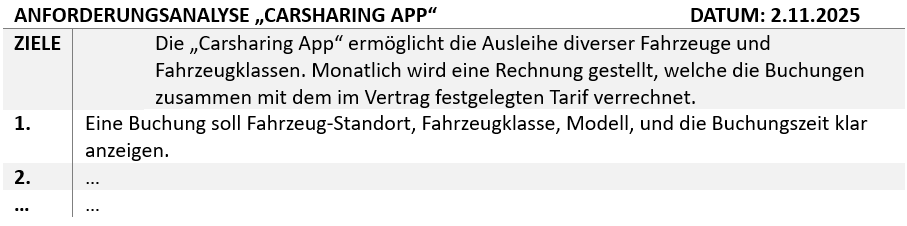
\includegraphics[width=\linewidth]{./pictures/Anforderungsliste}
	\caption{Eine für die theoretische Betrachtung der Datenbankmodellierung verkürzte Anforderungsanalyse der \glqq Carsharing Applikation\grqq.}
	\label{fig:Anforderungsanalyse}
\end{figure}

\subsection{Konzeptionelle Datenmodellierung}
Aus der Anforderungsanalyse wird das \textit{semantische Modell} in Form z.B. eines Entitaeten-Beziehungsmodells (Entity-Relationship-Modell, ERM) erarbeitet (\cite{gehringWirtschaftsinformatik2022}: 18). Ähnlich den Klassen in der objektorientierten Programmierung werden Entitäts-Typen festgelegt und mit bestimmten Eigenschaften (Attributen) definiert und gegenseitige Entitaets-Beziehungstypen abgeleitet. Die Beziehungstypen sind durch Assoziationen mengenmäßig verknüpft, sodass beispielsweise einem Kunden mehrere Rechnungen zugeordnet sein können, eine Rechnung jedoch nicht mehreren Kunden zugeordnet sein kann. Wie in \autoref{fig:ERM-Diagram-Definitionen} dargestellt, wurden für das ERM feste Symbole festgelegt um Entitätstypen (Rechteck), Beziehungstypen (Raute), Assoziationen (Pfeile) und Attribute (Kreise) darzustellen. Für die Darstellung der Assoziationen existieren mehrere Darstellungen, wobei sich diese Arbeit auf die ursprüngliche Chen-Notation (1:1, 1:n, n:1, n:m) beschränkt (\cite{gluchowskiDatenmodellierungDataWarehouseSystemenKonzepte2025}: 36).

\begin{figure}[htb]
	\centering
	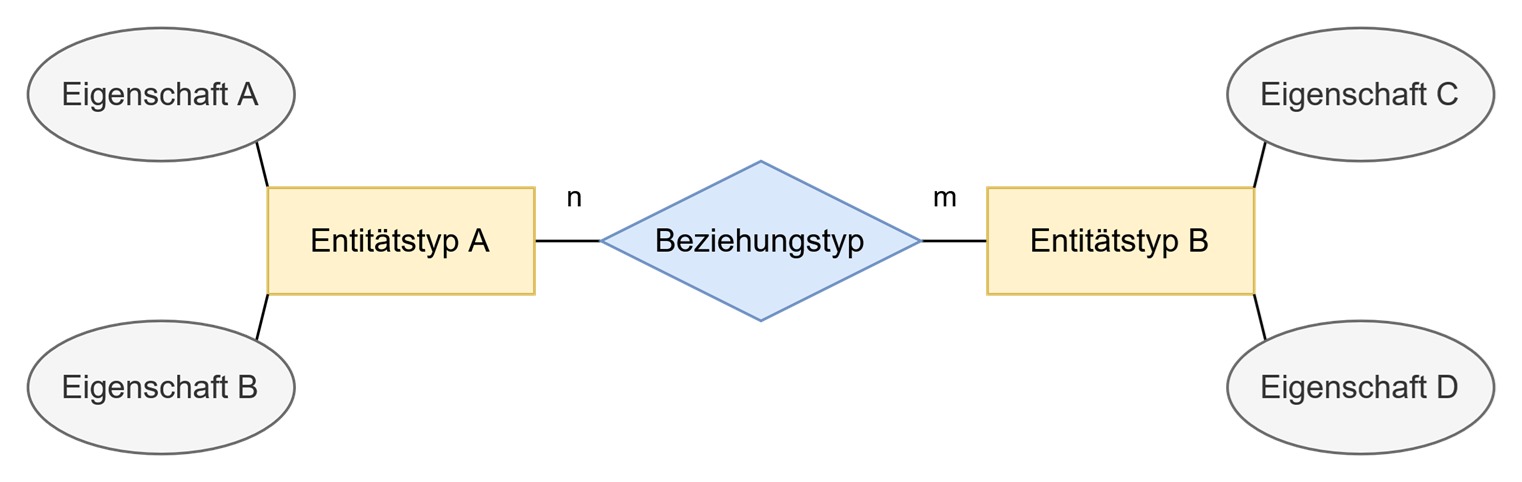
\includegraphics[width=\linewidth]{./pictures/ERM-Diagram-Definitionen}
	\caption{ERM-Darstellung für Entitätstypen (Rechteck), Beziehungstypen (Raute), Assoziationen (Pfeile) und Attribute (Kreise). Die Assoziationen sind in der Chen-Notation 1:1, 1:n, oder n:m dargestellt. Die Farben dienen nur der Übersichtlichkeit.}
	\label{fig:ERM-Diagram-Definitionen}
\end{figure}

Für das Beispiel der \glqq Carsharing Applikation\grqq\ sollen sich für das bessere Verständnis der nachfolgenden Schritte in der Datenmodellierung nur die Entitätstypen Kunde und Fahrzeug-Buchung ergeben. Die ausführliche Darstellung findet sich im Hauptteil dieser Arbeit.

\subsection{Abbildung auf Relationenmodell}
\label{subsec:Abbildung auf Relationenmodell}
Während das bisher betrachtete semantische Modell unabhängig war vom Datenbankmodell wird im logischen Schema ein spezifisches Modell festgelegt. In dieser Arbeit wird das Relationenmodell angewendet, welches Anfang der 1970er Jahre von Edgar Frank Codd begründet wurde. Dieser setzte sich unter anderem mit dem mathematisch-logischen Problem einer redundanzfreien Datenmodellierung auseinander (\cite{kaufmannSQLNoSQLDatenbanken92023}: 14).

In einer Veröffentlichung von 1970 beschrieb Codd (\cite{coddRelationalModelData1970}) bestimmte Regeln für die Erstellung und Optimierung einer Datenstruktur im relationalen Modell, die weiterhin gültig sind. Nach Codd bestehen relationale Datenstrukturen aus Relationen (engl. relations) auf Eigenschaften, die als Tupel (engl. set) definiert sind. Die einzelnen Elemente dieses Tupels nennt Codd auch Domänen (engl. domains) (\cite{coddRelationalModelData1970}: 379). Hieraus leitet sich direkt eine Zusammengehörigkeit dieser Eigenschaften zu einer Relation heraus, die man sich graphisch als Baumstruktur oder auch Tabelle vorstellen kann. Die Baumstruktur (vgl. Darstellung in \cite{coddRelationalModelData1970}: 379) bietet den Vorteil, dass \glqq non-simple domains\grqq\ übersichtlicher dargestellt werden können, während in Tabellen diese \glqq non-simple domains\grqq\ in weitere Relationen-Tabellen ausgegliedert und deren ursprüngliche Beziehungen durch Primär- und Fremdschlüssel festgehalten werden (\cite{kaufmannSQLNoSQLDatenbanken92023}: 41ff). Aufgrund der Komplexität der Datenmodellierung ist es sinnvoll, die verschiedenen Darstellungsformen und deren Einsatzgebiete zu verstehen.

Tabelle \ref{table:Buchung} zeigt die Relation \textit{Buchung} als vereinfachte Form für unser Beispiel einer \glqq Carsharing Applikation\grqq (im Hauptteil weiter ausgeführt). Das Tupel, das die Eigenschaften festlegt lautet (ID, Buchungszeit, Fahrzeug, Standort).  Zeilenweise werden darunter Datensätze dargestellt, wobei die Zeilenreihenfolge (im Gegensatz zur Reihenfolge der Spalten) egal ist. In jeder Relation wird ein Primärschlüssel festgelegt, der jeden Eintrag eindeutig festlegt und nicht doppelt vorkommen kann. Wichtig ist nur die Eindeutigkeit, daher ist auch eine Kombination von Attributen möglich, die einzeln nicht eindeutig sind, aber in Kombination nur ein Mal auftreten. Hierbei ist zu beachten, dass diese Kombination auch in einer wachsenden Tabelle immer noch eindeutig sein muss, weswegen es oft einfacher sein kann eine eindeutige ID für neue Einträge zu vergeben. Im Beispiel wird eine solche ID als Primärschlüssel verwendet.

\begin{table}[htb]
	
	\centering
	\caption{Buchung}\label{table:Buchung}
	\begin{tabular}{llllllll} \toprule
		ID & Buchungszeit & Fahrzeug & Standort \\ 
		\midrule
		000 & 14.10.25, 15:00-17:00 & Touran, M & Amselweg 15, 8888 Musterstadt \\
		003 & 11.03.22, 08:00-11:00 & Multivan, L & Spatzengasse 26, 7777 Musterhausen \\
		001 & 25.09.25, 11:00-17:00 & Punto, S & Möweninsel 13, 7777 Musterhausen \\
		004 & 25.09.25, 11:00-17:00 & Twingo, S & Möweninsel 13, 7707 Musterhausen \\
		\bottomrule
	\end{tabular}
\end{table}


Die redundanzarme Datenmodellierung erfolgt in mehreren Schritten die Codd als \textit{Normalisierung} bezeichnete: "There is, in fact, a very simple elimination procedure, which we shall call normalization\  (\cite{coddRelationalModelData1970}: 381)". Nachfolgend sollen die drei Formen der Normalisierung auf die Tabelle \ref{table:Buchung} beispielhaft angewendet werden.

\paragraph{1. Normalform}
Eine Relation befindet sich in der 1. Normalform, wenn alle Attribute atomare, d.h. nicht weiter unterteilbare Attributausprägungen aufweisen (\cite{gehringWirtschaftsinformatik2022}: 798). In Tabelle \ref{table:Buchung} zeigt sich, dass das Attribut Fahrzeug neben dem Fahrzeugnamen auch die Fahrzeugklasse enthält, wobei unterschiedliche Fahrzeugnamen der gleichen Klasse zugeordnet sind. Zudem findet sich eine Doppelung der Einzel-Einträge von \glqq Adresse, Hausnummer, PLZ, Stadt\grqq\ bei der Kategorie Standort. Durch Aufteilung in eigene Attribute ergibt sich daher die 1. Normalform in Tabelle \ref{table:1NF:Buchung}.

\begin{table}[!ht]
	
	\centering
	\caption{Buchung (1.Normalform)}\label{table:1NF:Buchung}
	\begin{tabular}{llllllll} \toprule
		ID 	& Buchungszeit & Fahrzeug & Typ & Stra\ss e & Nr & PLZ & Stadt \\ 
		\midrule
		000 & 14.10.25 15:00-17:00 & Touran & M & Amselweg & 15 & 8888 & Musterstadt \\
		003 & 11.03.22 08:00-11:00 & Multivan & L & Spatzengasse & 26 & 7777 & Musterhausen \\
		001 & 25.09.25 11:00-17:00 & Punto & S & Möweninsel & 13 & 7777 & Musterhausen \\
		004 & 25.09.25 11:00-17:00 & Twingo & S & Möweninsel & 13 & 7707 & Musterhausen \\
		\bottomrule
	\end{tabular}
\end{table}

\paragraph{2. Normalform}
Ausgehend von einer Relation, die sich bereits in der 1. Normalform befindet, ergibt sich die 2. Normalform wenn jedes Nichtschlüsselattribut vom Identifikationsschlüssel voll-funktional abhängig ist. (\cite{gehringWirtschaftsinformatik2022}: 799). In der Relation Buchung (\autoref{table:1NF:Buchung}) ist die Buchungs-ID der Primärschlüssel und das Attribut Buchungszeit voll-funktional von diesem abhängig. Die weiteren Attribute sind jedoch nur teil-funktional von der Buchungs-ID abhängig. Fahrzeug und Typ sind stattdessen voll-funktional abhängig von einem bestimmten Fahrzeug (\autoref{table:2NF:Fahrzeug}) und die Stra\ss e, Nr, PLZ und Stadt sind nur voll-funktional abhängig von einem bestimmten Standort des Fahrzeugs (siehe \autoref{table:2NF:Standort}). Die Auflösung dieser teil-funktionalen Abhängigkeiten erfolgt durch die Aufspaltung in separate Relationen (Tabellen). Die Verbindung der Relationen wird durch Fremdschlüssel definiert, die beispielsweise in der Relation Buchung (\autoref{table:2NF:Buchung}) das Fahrzeug und den Standort des Fahrzeugs festhalten. Zur Kennzeichnung werden die Primärschlüssel und Fremdschlüssel unterstrichen. Fremdschlüssel wurden in dieser Arbeit außerdem kursiv geschrieben.

\begin{table}[!ht]
	\centering
	\caption{Buchung (2. Normalform)}\label{table:2NF:Buchung}
	\begin{tabular}{llllllll} \toprule
		\underline{Buchungs-ID} & Buchungszeit & \textit{\underline{Fahrzeug}} & \textit{\underline{Standort}}	 \\ 
		\midrule
		000&  14.10.25 15:00-17:00  & R-AA-123 & 000 \\
		003&   11.03.22 08:00-11:00 & M-XY-321 & 001  \\
		001&   25.09.25 11:00-17:00 & M-QE-355 & 002  \\
		004&   25.09.25 11:00-17:00 & M-SR-411 & 003  \\
		\bottomrule
	\end{tabular}
%\end{table}

%\begin{table}
	\parbox{.35\linewidth}{
	\centering
	\caption{Fahrzeug (2. Normalform)}\label{table:2NF:Fahrzeug}
	\begin{tabular}{lll} \toprule
		\underline{Fahrzeug} 	& Modell & Typ \\ 
		\midrule
		R-AA-123 & Touran & M    \\
		M-XY-321 & Multivan & L  \\
		M-QE-355 & Punto & S     \\
		M-SR-411 & Twingo & S    \\
		\bottomrule
	\end{tabular}
	}
	\hfill
	\parbox{.62\linewidth}{
	\centering
	\caption{Standort (2. Normalform)}\label{table:2NF:Standort}
	\begin{tabular}{lllll} \toprule
	\underline{Standort} 	& Stra\ss e & Nr & PLZ & Stadt \\ 
	\midrule
	000 & Amselweg & 15 & 8888 & Musterstadt \\
	001 & Spatzengasse & 26 & 7777 & Musterhausen \\
	002 & Möweninsel & 13 & 7777 & Musterhausen \\
	003 & Möweninsel & 13 & 7707 & Musterhausen \\
	\bottomrule
\end{tabular}
	}
\end{table}

\paragraph{3. Normalform}
Ausgehend von einer Relation die sich bereits in der 2. Normalform befindet, ergibt sich die 3. Normalform wenn kein Attribut transitiv vom Primärschlüsselattribut abhängt. In der Tabelle \ref{table:2NF:Standort} ist die Stadt primär abhängig von der PLZ. Eine Stadt kann mehrere PLZ besitzen, jedoch ist jede PLZ eindeutig einer Stadt zugehörig. Die Stadt ist daher nur transitiv vom Primärschlüssel des Standorts abhängig. Eine Auflösung dieser inneren Redundanz kann durch die Aufspaltung von \autoref{table:2NF:Standort} in eine weitere Relation Ortsnamen (\autoref{table:3NF:Ortsname}) erfolgen, in welcher die PLZ mit den Ortsnamen verknüpft sind. Die Relation zur \autoref{table:3NF:Ortsname} wird in dieser durch den Fremdschlüssel PLZ mit \autoref{table:3NF:Standort} verknüpft.

\begin{table}[ht]
	\parbox{.5\linewidth}{
	\centering
	\caption{Standort (3. Normalform)}
	\label{table:3NF:Standort}
	\begin{tabular}{lllll} \toprule
		\underline{Standort} 	& Stra\ss e & Nr & \textit{\underline{PLZ}}\\ 
		\midrule
		000 & Amselweg & 15 & 8888 \\
		001 & Spatzengasse & 26 & 7777 \\
		002 & Möweninsel & 13 & 7777 \\
		003 & Möweninsel & 13 & 7707 \\
		\bottomrule
	\end{tabular}
	}
	\hfill
	\parbox{.5\linewidth}{
		\centering
		\caption{Ortsname (3. Normalform)}
		\label{table:3NF:Ortsname}
		\begin{tabular}{ll} \toprule
			\underline{PLZ} 	& Stadt \\ 
			\midrule
			8888 & Musterstadt \\
			7777 & Musterhausen \\
			7777 & Musterhausen \\
			7707 & Musterhausen \\
			\bottomrule
		\end{tabular}
	}
\end{table}

Insbesondere der letzte Normalisierungsschritt in dem Beispiel zeigt, dass es nicht immer sinnvoll ist, die Regeln der Normalisierung beim Datenbankentwurf strikt zu befolgen. Die Ausgliederung des Ortsnamens erzeugt eine zusätzliche Tabelle die über einen zusätzlichen Fremdschlüssel gespeichert und bei einer Abfrage zusätzlich abgerufen werden muss. Allgemein bietet die Codd'sche Normalisierung jedoch eine gute Grundlage, um ausgehend von einer möglichst redundanzfreien Struktur nur die Redundanzen aufzulösen, welche die anfänglich genannten Ziele einer geringen Redundanz, guten Bedienbarkeit, flexiblen Erweiterbarkeit, hohen Performance, der Konsistenz und Integrität bestmöglich erfüllen.

Ausgehend von dieser theoretischen Betrachtung einer Datenbankmodellierung wird im nächsten Kapitel die vollständige Datenbank einer potentiellen \glqq Carsharing App\grqq\ entworfen und beispielhaft gezeigt, wie die Daten in einem Datenbankverwaltungssystem mittels der Datenbanksprache SQL abgerufen und bearbeitet werden können.












\section{Hauptteil}
\label{section:main}

Im Hauptteil dieser Arbeit wird die \glqq Carsharing Applikation\grqq anhand der im Theorieteil beschriebenen Entwurfsschritte: 1. Anforderungsanalyse, 2. ERM, und 3. Abbildung auf Relationenmodell entworfen. Anschließend wird die Datenbank in Racket übertragen und beispielhaft gezeigt, wie mit der Datenbanksprache SQL einzelne Datensätze erstellt und abgerufen werden können.

\subsection{Datenbankmodell einer \glqq Carsharing Applikation\grqq}

\paragraph{Schritt 1: Anforderungsanalyse}
In \autoref{fig:Anforderungsanalyse_Main} ist eine ausführliche Anforderungsanalyse der \glqq Carsharing Applikation\grqq dargestellt. Aus diesen Anforderungen können nun die Entitäten (Klassen), ihre Attribute und die Beziehungen abgeleitet und in ein ERM übertragen werden.

\begin{figure}[htb]
	\centering
	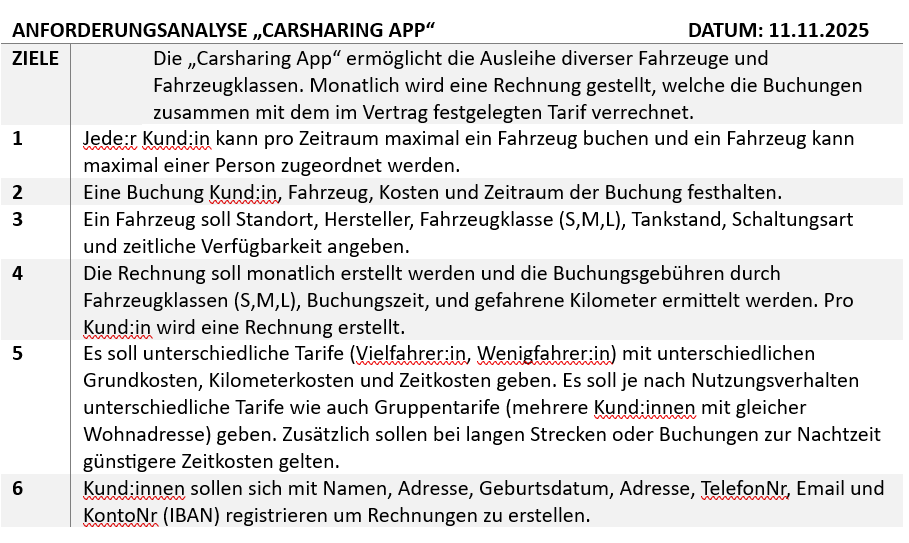
\includegraphics[width=\linewidth]{./pictures/Anforderungsliste_Main}
	\caption{Anforderungsanalyse für die \glqq Carsharing Applikation\grqq.}
	\label{fig:Anforderungsanalyse_Main}
\end{figure}

\paragraph{Schritt 2: Abbildung in ein ERM}
Für das ERM werden die relevanten Entitäten und Beziehungstypen aus dem Anforderungskatalog abgeleitet. Auf Basis des Anforderungskatalogs in \autoref{fig:Anforderungsanalyse_Main} ergeben sich Kund:in, Fahrzeug, Fahrzeugklasse, Buchung, Tarif, Vertrag, Rechnung, Rechnungsposition und Adresse als Entitätstypen. Zwischen diesen Entitätstypen ergeben sich folgende Beziehungstypen und Assoziationen:
\begin{itemize}[itemsep=3pt]
	\item Kund:in $\rightarrow$ n besitzt 1     $\rightarrow$ Vertrag
	\item Kund:in     $\rightarrow$ 1 führt aus n     $\rightarrow$ Buchung
	\item Kund:in     $\rightarrow$ 1 erhält n     $\rightarrow$ Rechnung
	\item Kund:in     $\rightarrow$ n wohnt in 1     $\rightarrow$ Wohn-Adresse
	\item Buchung     $\rightarrow$ 1 erstellt 1     $\rightarrow$ Rechnungsposition
	\item Buchung     $\rightarrow$ 1 mietet 1     $\rightarrow$ Fahrzeug
	\item Rechnungsposition     $\rightarrow$ n wird abgerechnet 1     $\rightarrow$ Rechnung
	\item Vertrag     $\rightarrow$ n nutzt 1     $\rightarrow$ Tarif
	\item Fahrzeug     $\rightarrow$ n besitzt 1     $\rightarrow$ Standort-Adresse
	\item Fahrzeug     $\rightarrow$ n gehört zu 1     $\rightarrow$ Fahrzeugklasse
\end{itemize}
Es fällt auf, dass Wohn-Adresse (Kund:in) und Standort-Adresse (Fahrzeug) beides Adressen sind. Diese Ähnlichkeit wird als gemeinsamer Entitätstyp \glqq Adresse\grqq\ zusammengeführt. Die graphische Darstellung dieser Entitätstypen, Beziehungstypen, Assoziationen und Attribute zeigt das ER-Diagramm in \autoref{fig:ERM_Carsharing}. Hier sind die Primärschlüsselattribute durch Unterstreichen gekennzeichnet.

\begin{figure}[htb]
	\centering
	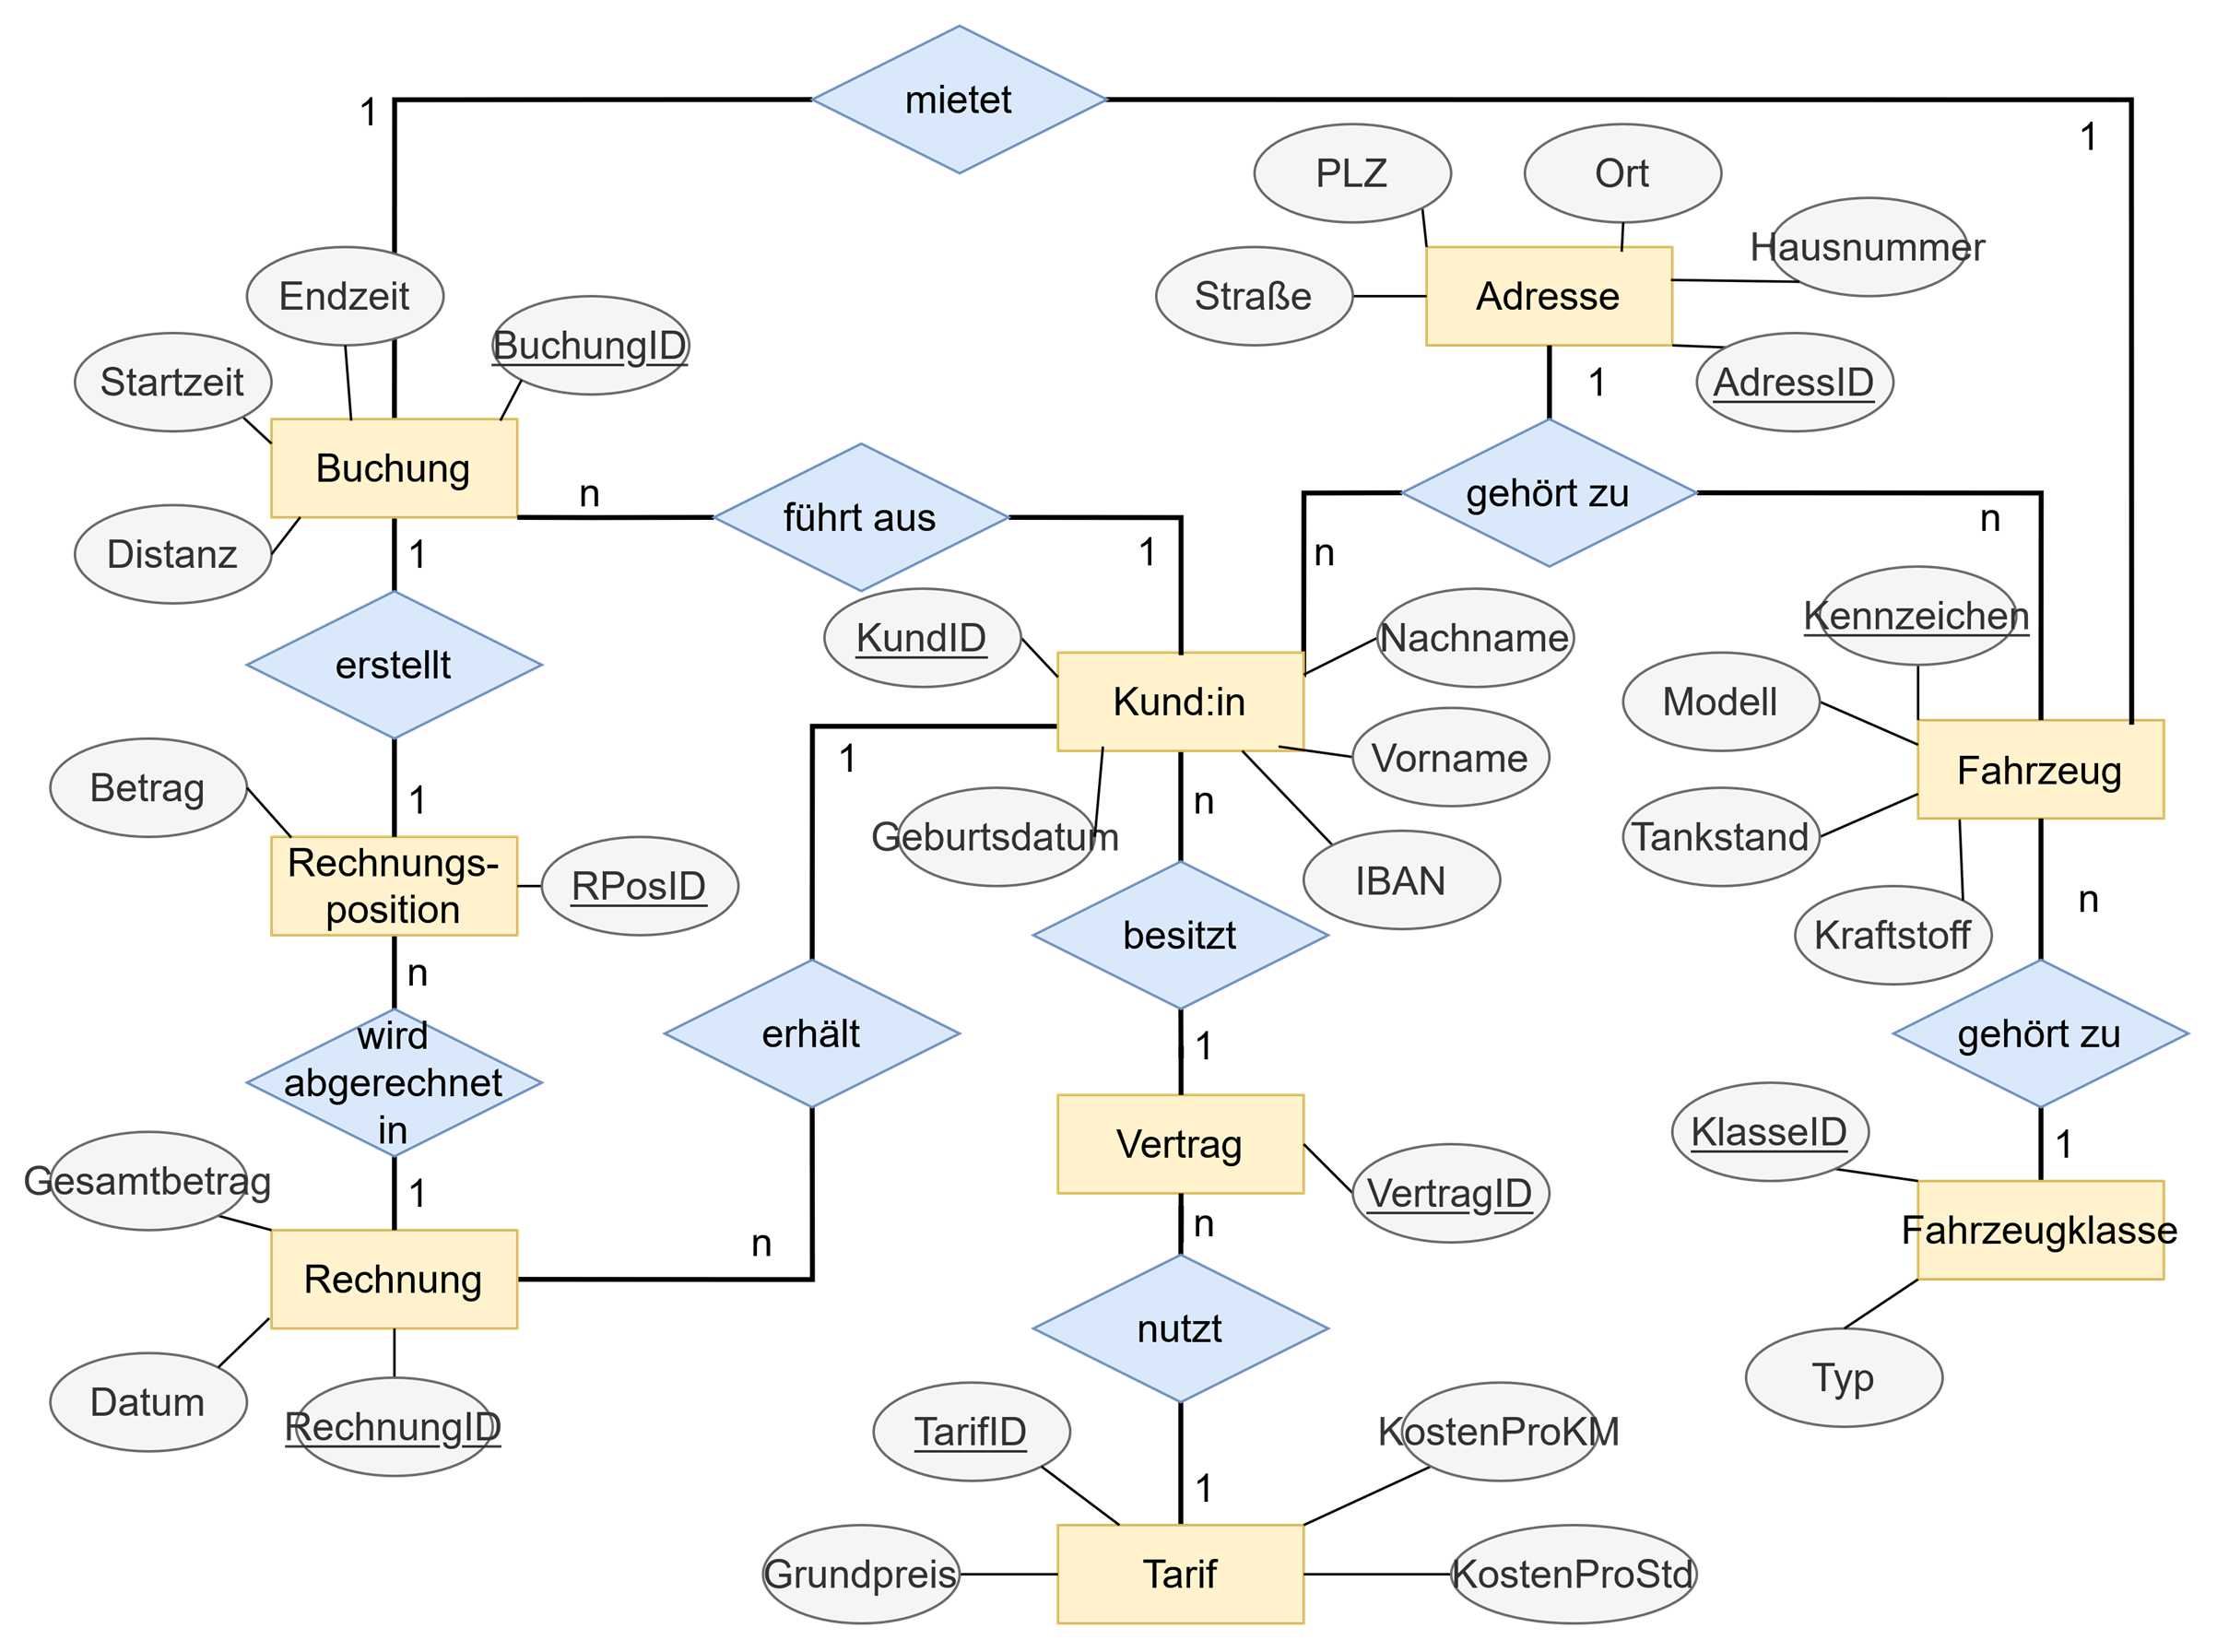
\includegraphics[width=\linewidth]{./pictures/ERM_Carsharing}
	\caption{ERM-Diagramm von der \glqq Carsharing Applikation\grqq.}
	\label{fig:ERM_Carsharing}
\end{figure}

In dem Entwurf des ER-Diagramms war insbesondere die Definition der Beziehungen eine gro\ss e Herausforderung. Die Beziehungen werden im nachfolgenden Relationenmodell in Fremdschlüssel übersetzt und sollten nur dort festgelegt werden, wo sie zwingend für die Definition der Entität notwendig sind. Beispielsweise wäre eine Buchung ohne die Festlegung eines Fahrzeugs nicht sinnhaft, weswegen in der Buchung eine Beziehung zu Fahrzeug definiert sein muss. In der späteren Umsetzung in eine reale Datenbank ist es sinnvoll programmatisch festzulegen, dass Datensätze ohne gültige Fremdschlüssel gar nicht erst angelegt werden dürfen. Dies stellt sicher, dass die Abfrage von Daten immer ein erwartetes Ergebnis liefert.

\paragraph{Schritt 2: Abbildung auf Relationenmodell}
Das ERM wird nun auf das Relationenmodell als spezifische Datenbankstruktur abgebildet. Für jeden Entitätstyp wurde in \ref{table:Buchung_main} bis \ref{table:Fahrzeugklasse_main} aus dem ER-Diagramm (\autoref{fig:ERM_Carsharing}) die entsprechende Tabelle erstellt. Hierbei wurden die Regeln der Normalisierung (siehe \autoref{subsec:Abbildung auf Relationenmodell}) bereits auf die Tabellen angewendet. Die einzelnen Datensätze (Entitäten) wurden in den Tabellen aus Gründen der Übersichtlichkeit nur durch Punkte angedeutet. Die Datensätze werden nachfolgend stattdessen im XML Format angegeben, das sich für die Darstellung besser eignet.

\begin{table}
	\centering
	\caption{Buchung}\label{table:Buchung_main}
	\begin{tabular}{l l l l l l} \toprule
		\underline{BuchungID} & Startzeit & Endzeit & Distanz & \textit{\underline{Kennzeichen}} & \textit{\underline{KundID} 	} \\ 
		\midrule
		\dots &  \dots & \dots  & \dots & \dots & \dots \\
		\bottomrule
	\end{tabular}
%\end{table}

%\begin{table}
	\centering
	\caption{Rechnung}\label{table:Rechnung_main}
	\begin{tabular}{l l l l l} \toprule
		\underline{RechnungID}  & Gesamtbetrag & Datum & \textit{\underline{KundID}} &  \textit{\underline{RPosID}}  \\ 
		\midrule
		\dots &  \dots & \dots  & \dots & \dots  \\
		\bottomrule
	\end{tabular}
%\end{table}

%\begin{table}
	\parbox{.49\linewidth}{
		\centering
		\caption{Rechnungsposition}\label{table:Rechnungsposition_main}
		\begin{tabular}{l l l} \toprule
			\underline{RPosID} & Betrag & \textit{\underline{BuchungID}} \\ 
			\midrule
			\dots &  \dots \\
			\bottomrule
		\end{tabular}
	}
	\parbox{.49\linewidth}{
		%\begin{table}
		\centering
		\caption{Adresse}\label{table:Adresse_main}
		\begin{tabular}{l l l l l} \toprule
			\underline{AdressID} & Stra\ss e & Nr & PLZ & Ort \\ 
			\midrule
			\dots &  \dots & \dots  & \dots & \dots \\
			\bottomrule
		\end{tabular}
		%\end{table}
	}
%\end{table}

%\begin{table}
	\centering
	\caption{Kund:in}\label{table:Kund_main}
	\begin{tabular}{l l l l l l} \toprule
	\underline{KundID} 	& Vorname & Nachname & Geburtsdatum & IBAN & \textit{\underline{AdressID}} \\ 
	\midrule
	\dots &  \dots & \dots  & \dots & \dots & \dots \\
	\bottomrule
	\end{tabular}
%\end{table}

%\begin{table}
	\centering
	\caption{Tarif}\label{table:Tarif_main}
	\begin{tabular}{l l l l} \toprule
		\underline{TarifID} & Grundpreis & KostenProKM & KostenProStd \\ 
		\midrule
		\dots &  \dots & \dots  & \dots  \\
		\bottomrule
	\end{tabular}
%\end{table}

%\begin{table}
	\parbox{.45\linewidth}{
		\centering
		\caption{Vertrag}\label{table:Vertrag_main}
		\begin{tabular}{l l l l} \toprule
		\underline{VertragID} &  \textit{\underline{KundID}} & \textit{\underline{TarifID}} \\ 
		\midrule
		\dots &  \dots & \dots  \\
		\bottomrule
		\end{tabular}
	}
	\parbox{.45\linewidth}{
		\centering
		\caption{Fahrzeugklasse}\label{table:Fahrzeugklasse_main}
		\begin{tabular}{l l} \toprule
			\underline{KlasseID} & Typ\\ 
			\midrule
			\dots &  \dots \\
			\bottomrule
		\end{tabular}
	}
%\end{table}

%\begin{table}
	\centering
	\caption{Fahrzeug}\label{table:Fahrzeug_main}
	\begin{tabular}{l l l l l l} \toprule
		\underline{Kennzeichen} & Modell & Tankstand & Kraftstoff &  \textit{\underline{KlasseID}} & \textit{\underline{AdressID}} \\ 
		\midrule
		\dots &  \dots & \dots  & \dots &  \dots & \dots  \\
		\bottomrule
	\end{tabular}
\end{table}

Die folgende XML codierte Darstellung zeigt einen Datensatz aus der Tabelle \textit{Rechnung}. Das XML Format erlaubt eine hierarchische Darstellung von Datensätzen. Dadurch können Sichtweisen, aus denen heraus die Datensätze betrachtet werden übersichtlich dargestellt werden. Die gewählte Sichtweise, aus der ein Datensatz in XML dargestellt wird, bestimmt die logische bzw. hierarchische Struktur der verknüpften Entitäten. Für den XML-Codeausschnitt wurde die Sichtweise der Beispiel-Rechnung \glqq R1B3C\grqq) gewählt, sodass Kunde \glqq K100A\grqq\ und Rechnungspositionen \glqq P2341G\grqq, \glqq PAB234\grqq als untergeordnete Fremdschlüssel-Attribute auftauchen. Wie im ERM-Diagramm in \autoref{fig:ERM_Carsharing} dargestellt sind diese durch Fremdschlüssel verknüpften Informationen wichtig für den Vorgang der Rechnungserstellung. Analog würden sich für die anderen Entitäten sehr unterschiedliche Sichtweisen und somit Darstellungen der primären Attribute, sowie sekundärer über Fremdschlüssel verknüpfter Attribute ergeben. Eine flache Darstellung von Datensätzen im XML Format ohne Hierarchien ist im Anhang (\autoref{subsec:XMLcode}) dargestellt und bildet alle Datensätze ab für das beispielhaft erstellte DMBS erstellt wurden.

\begin{lstlisting}[language=XML]
<?xml version="1.0" encoding="UTF-8"?>
<CarsharingDatensaetze>
    <!--Beispieldatensatz Rechnung?-->
    <RechnungID id="R1B3C">
        <Gesamtbetrag>123.34</Gesamtbetrag>
        <Datum>Schmidt</Datum>
        <KundID id="K100A">
            <Vorname>Ralf</Vorname>
            <Nachname>Hanser</Nachname>
            <Geburtsdatum>13.04.1999</Geburtsdatum>
            <IBAN>DE89370400440532013000</IBAN>
            <VertragID id="V2361C">
                <...>
            </VertragID>
            <AdressID id="A2361C">
                <...>
            </AdressID>
        </KundID>
        <RPosID id="P2341G">
            <Betrag>33.50</Betrag>
            <BuchungID id="B34DG">
        </RPosID>
        <RPosID id="PAB234">
            <Betrag>89.84</Betrag>
            <BuchungID id="C3123">
        </RPosID>
    </RechnungID>
</CarsharingDatensaetze>
\end{lstlisting}


\subsection{Datensätze in SQLite und Racket}
%Definieren Sie die Klassen auch als Code in Racket oder in einer anderen objektorientierten Programmiersprache. Die Beziehungen zwischen den Klassen müssen Sie nicht darstellen, dürfen Sie aber.
Die theoretischen Betrachtungen werden in diesem Abschnitt in ein relationales DBMS übertragen. Für die Realisierung wird die Programmiersprache Racket zusammen mit dem in Racket bereits implementierten DBMS SQLite verwendet. Der komplette Programm-Code (in Racket) um das DBMS in der entworfenen Form umzusetzen ist im Anhang in \autoref{subsec:SQLcode} gegeben. Beispielhaft wird dort auch ein Datensatz komplett angelegt und Beispielabfragen in SQL ausgeführt.

Zunächst wird eine SQlite Datenbank-Datei (.db) namens \glqq carsharing.db\grqq\ erstellt. Der Befehl \ir{PRAGMA foreign\_keys = ON} stellt sicher, dass Fremdschlüssel-Attribute erst definiert werden können wenn der Datensatz auf den sie verweisen existiert.
\begin{lstlisting}[language=racketSQL]
#lang racket
;; Carsharing Example: Connecting to SQLite ;; 
(require db)
;; Connect to (or create) a database file named "carsharing.db" ;;
(define conn
    (sqlite3-connect #:database "carsharing.db"
                     #:mode 'create))
;; Enable foreign key enforcement ;;
(query-exec conn "PRAGMA foreign_keys = ON;")
\end{lstlisting}

Über das \glqq conn\grqq\ Objekt kann die Datenbank beschrieben werden. Zunächst müssen die Entitätstypen über den Befehl \ir{CREATE TABLE} definiert werden. Die Definition der Attribute erfolgt zeilenweise über die Definition von Attributsname Datentyp und weiteren Typ-Eigenschaften. Das Schlüsselwort \ir{PRIMARY KEY} markiert den Primärschlüssel. Fremdschlüssel werden über die \ir{FOREIGN KEY} Definition in einer weiteren Zeile mit ihrer Referenz auf die Fremd-Tabelle definiert. Zusätzlich findet sich in der letzten Zeile das Schlüsselwort \ir{UNIQUE(..)}, welches festlegt, dass neben dem Primärschlüssel auch die Kombination aus den hier definierten Feldern nicht dupliziert vorliegen darf. Dadurch werden Duplikatseinträge verhindert, die durch den Befehl \ir{AUTOINCREMENT} im Primärschlüssel durch wiederholtes Anlegen von gleichen Einträgen entstehen können.
\begin{lstlisting}[language=racketSQL]
;; Create <Buchung> table ;; 
(query-exec conn
	"CREATE TABLE IF NOT EXISTS Buchung (
		id INTEGER PRIMARY KEY AUTOINCREMENT,
		startzeit TEXT NOT NULL,
		endzeit TEXT NOT NULL,
		distanz REAL,
		FahrzeugID TEXT NOT NULL,
		KundID INTEGER NOT NULL,
		FOREIGN KEY(FahrzeugID) REFERENCES Fahrzeug(Kennzeichen),
		FOREIGN KEY(KundID) REFERENCES Kunde(KundID),
		UNIQUE(startzeit, FahrzeugID, KundID)
		);")
\end{lstlisting}

Die Tabelle wird nun mit den Schlüsselwörtern \ir{INSERT ... INTO} mit Datensätzen gefüllt. \ir{IGNORE} oder \ir{REPLACE} verhindern das Erstellen von Duplikaten. Racket erlaubt das Verwenden von Platzhalter Argumenten \glqq ?\grqq\, welche in dem folgenden Beispiel verwendet wurden und die Übersichtlichkeit verbessern\footnote{Weitere Gründe für Platzhalter Argumente finden sich in der Racket Dokumentation: https://docs.racket-lang.org/sql/index.html, Zugriff am 28.11.2025}.
\begin{lstlisting}[language=racketSQL]
;; "Insert entry in <Buchung> table" ;;
(query-exec conn
	"INSERT OR IGNORE INTO Buchung (startzeit, endzeit, distanz, FahrzeugID, KundID)
	VALUES (?, ?, ?, ?, ?)"
	"2025-05-29 14:16:00" "2025-11-30 18:16:00" 15.30 "RO-CJ-262" 1)
\end{lstlisting}

Beispielhaft sollen nun Abfragen der Datenbank gezeigt werden. Abfragen werden in Racket über die \glqq conn\grqq\ Schnittstelle mittels der SQLite Syntax erstellt. Um die Abfrageergebnisse nachvollziehen zu können sind die Datensätze, welche in der Carsharing Datenbank eingetragen wurden in \autoref{subsec:XMLcode} als XML Struktur dargestellt. Im nachfolgenden Programmcode sind zwei Abfragen des Typs: \ir{SELECT ... FROM ... INNER JOIN ... ON ...} gegeben, welche sich dafür eignen um die Spalten zweier Tabellen auf Basis einer Identität (hier Identität von Primärschlüsseln und Fremdschlüsseln) abzufragen. Die erste Abfrage verwendet die Tabelle Kunde und Buchung um herauszufinden welche Buchungen von welchen Kund:innen durchgeführt wurden. Die zweite Abfrage liefert alle Fahrzeuge mit ihren zugehörigen Standortadressen, so dass Kund:innen-Adressen nicht mit aufgeführt werden.
\begin{lstlisting}[language=racketSQL]
;; "Query bookings from all customers" ;;
(define Buchungseintraege
	(query-rows conn
		"SELECT Vorname, Nachname, IBAN, FahrzeugKennzeichen, distanz
		FROM Kunde
		INNER JOIN Buchung on Buchung.KundID = Kunde.KundID"))
(for ([r Buchungseintraege])
	(printf "~a\n" r))
;; "Query parking locations of cars only (w/o customer adresses)" ;;
(define FahrzeugAdressen
	(query-rows conn
		"SELECT Modell, Kennzeichen, Strasse, Nr, PLZ, Ort
		FROM Adresse
		INNER JOIN Fahrzeug on Fahrzeug.AdressID = Adresse.AdressID;"))
(for ([r FahrzeugAdressen])
	(printf "~a\n" r))
\end{lstlisting}

Über die \ir{printf} Funktion werden die Variablen (Racket-Typ Liste), welche die Ergebnisse der Abfragen speichern ausgegeben. Für die erste Abfrage der Buchungseinträge erhält man:
\begin{lstlisting}[language=racketSQL]
#(Thomas Gerrer DE89370400440532013000 RO-CJ-262 15.3)
\end{lstlisting}
Und für die zweite Abfrage:
\begin{lstlisting}[language=racketSQL]
#(Fiat Punto RO-CJ-262 Eisenhutstr. 60 72072 Tuebingen)
\end{lstlisting}

Die hier gezeigte Umsetzung der Carsharing App \glqq TeilAuto Neckaralb\grqq in SQLite und Racket zeigt nur eine oberflächliche Betrachtung, welche einen Einstieg in die Welt relationaler Datenbanksystemen geben soll. Viele Aspekte eines realen DBMS für eine solche Anwendung wurden hier nicht berücksichtigt. Im Abschluss dieser Arbeit werden die Ergebnisse dieser Arbeit zusammengefasst und die Aspekte diskutiert, die in einer realen Datenbank zusätzlich berücksichtigt werden sollten.































\section{Zusammenfassung und Fazit}
\label{section:summary}
\subsection{Zusammenfassung}

Das Ziel dieser Arbeit war es den vollständigen Entwurfsprozess einer Datenbank anhand eines selbstgewählten Beispiels - hier einer Carsharing-Applikation - zu erarbeiten. Im theoretischen Teil wurde der Entwurfsprozess an einem reduzierten Modell der Carsharing-Applikation von der anfänglichen Anforderungsanalyse, über den konzeptionellen Entwurf mittels Entity-Relationship-Modell, bis hin zum finalen DBMS (hier ein Relationenmodell) erläutert und gezeigt, welche Überlegungen und Methoden angewandt werden müssen, um die zentralen Ziele der Datenbankmodellierung -- geringe Redundanz, gute Bedienbarkeit, einfache Erweiterbarkeit, schneller Zugriff, Konsistenz, und Integrität -- schrittweise zu optimieren. Im praktischen Teil wurde der Modellierungsprozess anschließend auf die möglichst vollständig ausgeführte Carsharing-Applikation übertragen und mittels Racket und dem relationalen DBMS SQLite umgesetzt.

\subsection{Kritische Reflexion}

Bei der Ausarbeitung dieser Arbeit wurde deutlich, wie wichtig die anfänglich angewandten konzeptionellen Schritte im Datenbankentwurf sind, um ein relationales DBMS zu entwerfen und in einem realen DBMS umzusetzen. Angefangen bei der Anforderungsanalyse zeigte sich, dass die alleinige Perspektive aus Kundensicht -- wie sie beim Autor dieser Arbeit vorliegt -- nicht ausreicht um die Anforderungsanalyse vollständig abzubilden. Prozesse, die insbesondere die Mitarbeitenden der Buchhaltung oder auch den Service bei Reparaturen oder Kundenanfragen betreffen wurden teilweise gar nicht oder nur unvollständig abgebildet. Als Vorteil für die Ausarbeitung der Arbeit erwies sich die vergleichsweise geringe Komplexität des gewählten Beispiels im Vergleich zu einer realen Carsharing-Applikation. Diese geringe Komplexität erleichterte den konzeptionellen Entwurf im ERM als auch die Abbildung des ERMs in den Tabellen des relationalen DBMS. 

Bei der Datenbankmodellierung wurde trotz Durchführung der einzelnen Modellierungsschritte auch nach der Umsetzung des realen DBMS iterativ zwischen den einzelnen Modellierungsschritten gewechselt. Die verschiedenen Perspektiven der einzelnen Modellierungsebenen erleichterten die Übersicht über mögliche Schwachstellen oder Fehler im Datenbankdesign. Korrigiert wurden insbesondere die Entitätstypen und deren Beziehungstypen. Bei den Beziehungstypen lag die Schwierigkeit darin, sinnvolle, aber nicht unnötig definierte Fremdschlüsselattribute zu wählen. Es wurde deutlich, dass insbesondere für Einsteiger:innen eine gründliche Auseinandersetzung mit den Zielen der einzelnen Modellierungsschritte sehr hilfreich ist, um zeiteffizient und strukturiert ein reales DBMS umzusetzen. 

Schließlich ist noch zu erwähnen, dass wichtige Aspekte, die durch die Skalierung des DBMS auf eine reale Carsharing-Applikation, die Benutzerfreundlichkeit der Applikation, die intelligente Anbindung einer Fahrzeugflotte, als auch die Sicherheit hinsichtlich Daten- und Diebstahlschutz in dieser Ausarbeitung ausgelassen wurden.
\section{Anhang}
\label{section:appendix}
\subsection{Racket/SQL Programmcode für das Carsharing DBMS}
\label{subsec:SQLcode}
\begin{lstlisting}[language=racketSQL]
#lang racket

;; ------------------------------------------------------------ ;;
;; "Basic Example: Connecting to SQLite" ;;
;; ------------------------------------------------------------ ;;
(require db)

;; Connect to (or create) a database file named "carsharing.db" ;;
(define conn
	(sqlite3-connect #:database "carsharing.db"
					 #:mode 'create))
;; Enable foreign key enforcement ;;
(query-exec conn "PRAGMA foreign_keys = ON;")

;; ------------------------------------------------------------ ;;
;; Create database tables ;; 
;; ------------------------------------------------------------ ;;
(query-exec conn
	"CREATE TABLE IF NOT EXISTS Adresse (
		AdressID Integer PRIMARY KEY AUTOINCREMENT,
		Strasse TEXT NOT NULL,
		Nr Integer NOT NULL,
		PLZ Integer NOT NULL,
		Ort TEXT NOT NULL,
		UNIQUE(Strasse, Nr, PLZ)
		);")

(query-exec conn
	"CREATE TABLE IF NOT EXISTS Fahrzeugklasse (
		KlasseID Integer PRIMARY KEY AUTOINCREMENT,
		Typ TEXT NOT NULL,
		UNIQUE(Typ)
		);")

(query-exec conn
	"CREATE TABLE IF NOT EXISTS Fahrzeug (
		Kennzeichen TEXT PRIMARY KEY,
		Modell TEXT NOT NULL,
		Tankstand REAL NOT NULL,
		Kraftstoff TEXT NOT NULL,
		KlasseID TEXT NOT NULL,
		AdressID TEXT NOT NULL,
		FOREIGN KEY(KlasseID) REFERENCES Fahrzeugklasse(KlasseID),
		FOREIGN KEY(AdressID) REFERENCES Adresse(AdressID)
		);")

(query-exec conn
	"CREATE TABLE IF NOT EXISTS Tarif (
		TarifID Integer PRIMARY KEY AUTOINCREMENT,
		Grundpreis TEXT NOT NULL,
		KostenProKM REAL NOT NULL,
		KostenProStd REAL NOT NULL,
		UNIQUE(Grundpreis, KostenProKM, KostenProStd)
		);")

(query-exec conn
	"CREATE TABLE IF NOT EXISTS Kunde (
		KundID Integer PRIMARY KEY AUTOINCREMENT,
		Vorname TEXT NOT NULL,
		Nachname TEXT NOT NULL,
		IBAN TEXT NOT NULL,
		Geburtsdatum TEXT NOT NULL,
		AdressID Integer,
		FOREIGN KEY(AdressID) REFERENCES Adresse(AdressID)
		);")

(query-exec conn
	"CREATE TABLE IF NOT EXISTS Vertrag (
		VertragID Integer PRIMARY KEY AUTOINCREMENT,
		KundID Integer,
		TarifID Integer,
		FOREIGN KEY(KundID) REFERENCES Kunde(KundID),
		FOREIGN KEY(TarifID) REFERENCES Tarif(TarifID)
		);")

(query-exec conn
	"CREATE TABLE IF NOT EXISTS Buchung (
		id INTEGER PRIMARY KEY AUTOINCREMENT,
		startzeit TEXT NOT NULL,
		endzeit TEXT NOT NULL,
		distanz REAL,
		FahrzeugKennzeichen TEXT NOT NULL,
		KundID INTEGER NOT NULL,
		FOREIGN KEY(FahrzeugKennzeichen) REFERENCES Fahrzeug(Kennzeichen),
		FOREIGN KEY(KundID) REFERENCES Kunde(KundID),
		UNIQUE(startzeit, FahrzeugKennzeichen, KundID)
		);")

(query-exec conn
	"CREATE TABLE IF NOT EXISTS Rechnungsposition (
		id INTEGER PRIMARY KEY AUTOINCREMENT,
		Betrag REAL NOT NULL,
		BuchungID INTEGER NOT NULL,
		FOREIGN KEY(BuchungID) REFERENCES Buchung(id),
		UNIQUE(BuchungID)
		);")

(query-exec conn
	"CREATE TABLE IF NOT EXISTS Rechnung (
		id INTEGER PRIMARY KEY AUTOINCREMENT,
		Datum TEXT NOT NULL,
		Gesamtbetrag REAL NOT NULL,
		RPosID INTEGER NOT NULL,
		KundID INTEGER NOT NULL,
		FOREIGN KEY(RPosID) REFERENCES Rechnungsposition(id),
		FOREIGN KEY(KundID) REFERENCES Kunde(KundID),
		UNIQUE(Datum, KundID)
		);")

;; ------------------------------------------------------------ ;;
;; Fill tables with data sets ;;
;; ------------------------------------------------------------ ;;
(query-exec conn
	"INSERT OR IGNORE INTO Adresse (Strasse, Nr, PLZ, Ort)
	VALUES (?,?,?,?)"
	"Eisenhutstr." 50 72072 "Tuebingen")

(query-exec conn
	"INSERT OR IGNORE INTO Adresse (Strasse, Nr, PLZ, Ort)
	VALUES (?,?,?,?)"
	"Eisenhutstr." 60 72072 "Tuebingen")

(query-exec conn
	"INSERT OR IGNORE INTO Fahrzeugklasse (Typ)
	VALUES (?)"
	"S")

(query-exec conn
	"INSERT OR IGNORE INTO Fahrzeug (Kennzeichen, Modell, Tankstand, Kraftstoff, KlasseID, AdressID)
	VALUES (?, ?, ?, ?, ?, ?)"
	"RO-CJ-262" "Fiat Punto" 0.57 "Benzin" 1 2)

(query-exec conn
	"INSERT OR IGNORE INTO Tarif (Grundpreis, KostenProKM, KostenProStd)
	VALUES (?, ?, ?)"
	10.00 0.43 1.20)

(query-exec conn
	"INSERT OR IGNORE INTO Kunde (Vorname, Nachname, IBAN, Geburtsdatum, AdressID)
	VALUES (?, ?, ?, ?, ?)"
	"Thomas" "Gerrer" "DE89370400440532013000" "13.04.1999" 1)

(query-exec conn
	"INSERT OR IGNORE INTO Vertrag (KundID, TarifID)
	VALUES (?, ?)"
	1 1)

(query-exec conn
	"INSERT OR IGNORE INTO Buchung (startzeit, endzeit, distanz, FahrzeugKennzeichen, KundID)
	VALUES (?, ?, ?, ?, ?)"
	"2025-05-29 14:16:00" "2025-11-30 18:16:00" 15.30 "RO-CJ-262" 1)

;; ------------------------------------------------------------ ;;
;; Query 'Buchungseintraege' and 'Fahrzeugeintraege' and print to screen ;;
;; ------------------------------------------------------------ ;;
(define Buchungseintraege
(query-rows conn
	"SELECT id, distanz, FahrzeugKennzeichen, KundID FROM Buchung"))
(for ([r Buchungseintraege])
	(printf "~a\n" r))

(define Fahrzeugeintraege
(query-rows conn
	"SELECT Kennzeichen, Modell FROM Fahrzeug"))
(for ([r Fahrzeugeintraege])
	(printf "~a\n" r))
\end{lstlisting}

\subsection{XML Darstellung der in Racket beispielhaft definierten Datensätze}
\label{subsec:XMLcode}
\begin{lstlisting}[language=XML]
<database file="code/carsharing.db">
	<table name="Adresse">
		<row>
			<cell name="AdressID">1</cell>
			<cell name="Strasse">Eisenhutstr.</cell>
			<cell name="Nr">50</cell>
			<cell name="PLZ">72072</cell>
			<cell name="Ort">Tuebingen</cell>
		</row>
		<row>
			<cell name="AdressID">2</cell>
			<cell name="Strasse">Eisenhutstr.</cell>
			<cell name="Nr">60</cell>
			<cell name="PLZ">72072</cell>
			<cell name="Ort">Tuebingen</cell>
		</row>
	</table>
	<table name="Fahrzeugklasse">
		<row>
		<cell name="KlasseID">1</cell>
		<cell name="Typ">S</cell>
		</row>
	</table>
	<table name="Tarif">
		<row>
		<cell name="TarifID">1</cell>
		<cell name="Grundpreis">10.0</cell>
		<cell name="KostenProKM">0.43</cell>
		<cell name="KostenProStd">1.2</cell>
		</row>
	</table>
	<table name="Kunde">
		<row>
		<cell name="KundID">1</cell>
		<cell name="Vorname">Thomas</cell>
		<cell name="Nachname">Gerrer</cell>
		<cell name="IBAN">DE89370400440532013000</cell>
		<cell name="Geburtsdatum">13.04.1999</cell>
		<cell name="AdressID">1</cell>
		</row>
	</table>
	<table name="Vertrag">
		<row>
		<cell name="VertragID">1</cell>
		<cell name="KundID">1</cell>
		<cell name="TarifID">1</cell>
		</row>
	</table>
	<table name="Fahrzeug">
		<row>
		<cell name="Kennzeichen">RO-CJ-262</cell>
		<cell name="Modell">Fiat Punto</cell>
		<cell name="Tankstand">0.57</cell>
		<cell name="Kraftstoff">Benzin</cell>
		<cell name="KlasseID">1</cell>
		<cell name="AdressID">2</cell>
		</row>
	</table>
	<table name="Buchung">
		<row>
		<cell name="id">1</cell>
		<cell name="startzeit">2025-05-29 14:16:00</cell>
		<cell name="endzeit">2025-11-30 18:16:00</cell>
		<cell name="distanz">15.3</cell>
		<cell name="FahrzeugKennzeichen">RO-CJ-262</cell>
		<cell name="KundID">1</cell>
		</row>
	</table>
	<table name="Rechnungsposition"/>
	<table name="Rechnung"/>
</database>
\end{lstlisting}
	


\clearpage

\pagenumbering{Roman}
\setcounter{page}{\value{savedpage}}

% --- LIST OF REFERENCES ---
\renewcommand*{\UrlFont}{\rmfamily}
\printbibliography

% Glossar
%\newpage
%\printnoidxglossaries

\end{document}
